\documentclass[10pt]{article}

\usepackage{fullpage}
\usepackage{graphicx}
\usepackage{mathtools}
\usepackage{setspace}
\usepackage{mdwlist}
\usepackage[center,font=singlespacing]{caption}
\usepackage{subfig}
\usepackage{hyperref}
\onehalfspacing

\begin{document}
\title{Augmented Reality Image Processing System}
\author{Logan P. Williams \& Jos\'{e} E. Cruz Serrall\'{e}s}
\date{December 10, 2011}
\maketitle

\section*{Abstract}
We have implement an augmented reality system that can overlay a digital image on video of a real world environment. We read NTSC video from a video camera and store it in ZBT SRAM. A picture frame with colored markers on the corners is held in front of the camera. We then perform chroma-based object recognition to locate the coordinates of the corners. Using these coordinates, we apply a low-pass filter and a projective transformation to project an image onto the dimensions of the picture frame. We then output VGA video of the original captured image, with the processed image overlayed on top of the frame.

\newpage

\tableofcontents
\listoffigures

\newpage

\section{Overview}
The augmented reality image processing system, or {\tt augreal}, uses a four stage buffered image processing pipeline. Images from a video camera are captured into a memory buffer, which on the next frame, is partially overwritten by skewed, scaled, and rotated pixels from the last image buffer that was displayed on the VGA output. On the next frame, this overwritten buffer becomes the video output. There are seven primary modules of this system.

The {\tt clock\_gen} module is responsible for creating and phase synchronizing the clocks used by the rest of the system. Because we require a specific video clock frequency, and the amount of computation and memory accesses we must perform, it is necessary for {\tt augreal} to use three distinct clock domains: a video capture clock, at approximately 27 mhz, generated externally by the video camera, a memory clock at 50 mhz, and a video output clock at 25 mhz.

The {\tt memory\_interface} module handles reading and writing from the ZBT memory, abstracting these operations away from the other modules. This module is responsible for ``shifting'' the buffers as described above.

Raw video is read from the video camera by the {\tt ntsc\_capture} module, which also finds recognizes pixels that match the colors of the corners of the target frame. These pixels are read by the {\tt object\_recognition} module which finds the weighted center of mass of the frame corners. The {\tt LPF} module sends each pixel ``on-the-fly'' to the {\tt projective\_transform} module which then sends that pixel's new coordinates to the {\tt memory\_interface} module to be written. The {\tt vga\_write} module reads and transmits the VGA data to be generated by the video DAC.

\begin{figure}[h!]
\centering
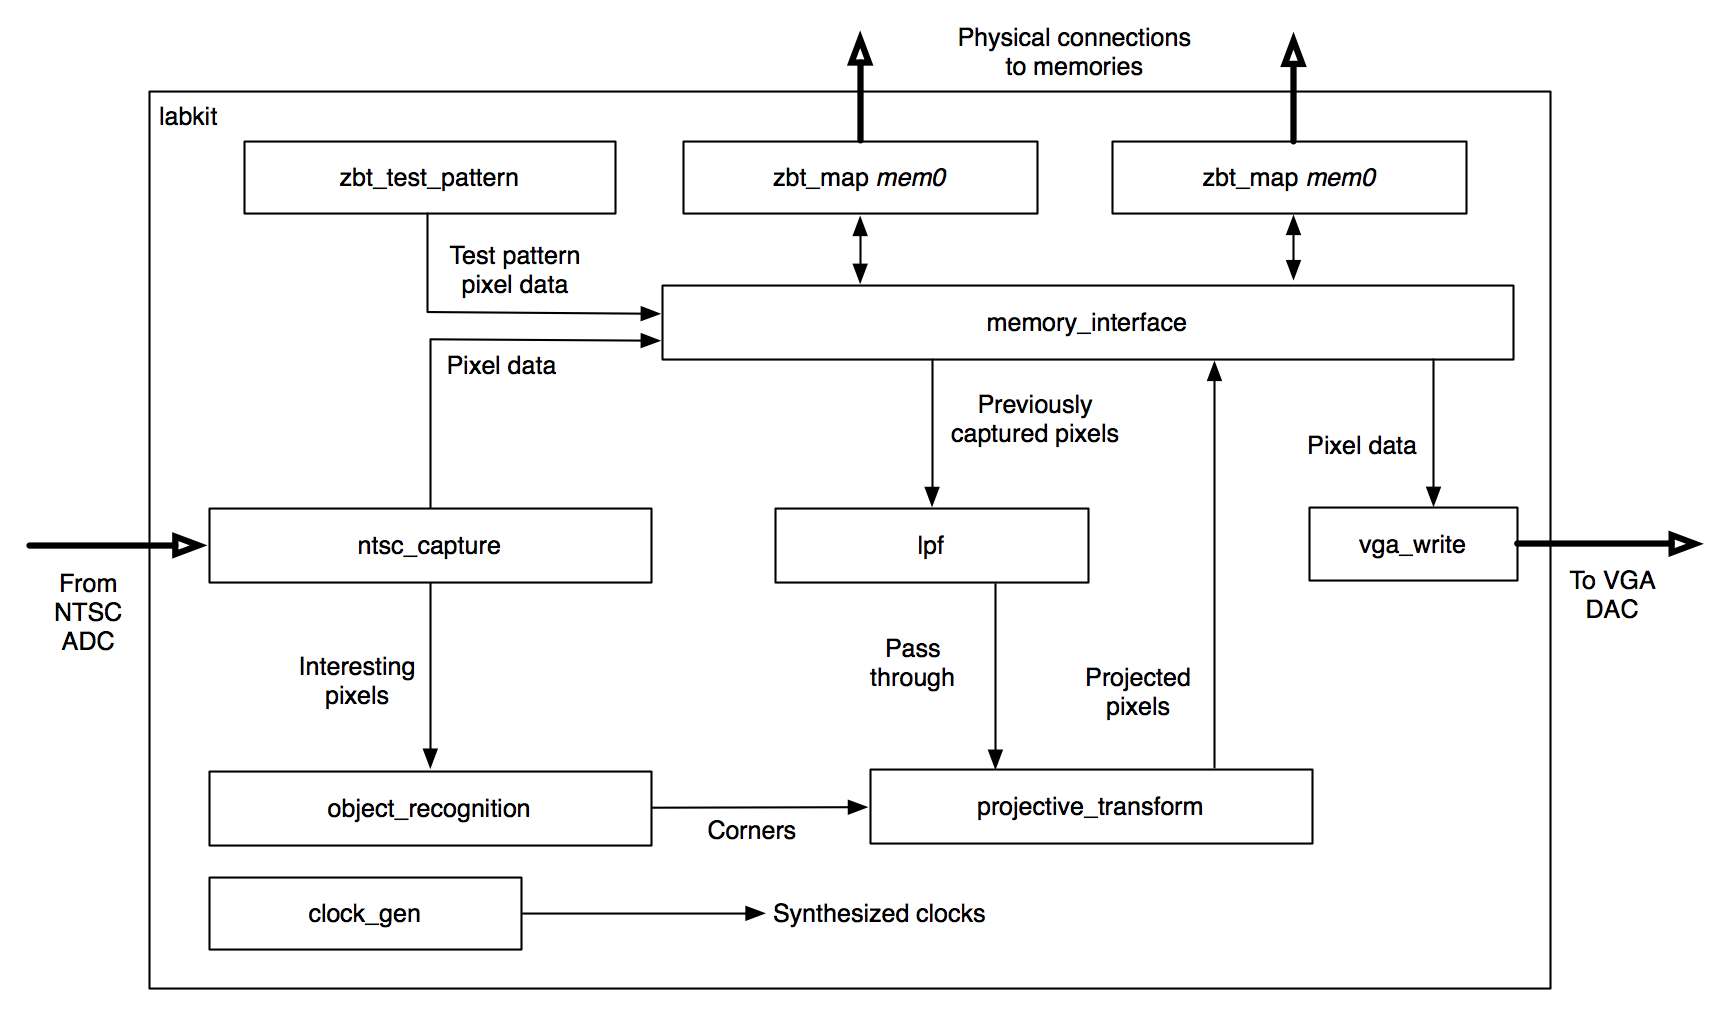
\includegraphics[width=\textwidth]{images/simplified_block_diagram.png}
\caption{\emph{An overview block diagram of the augmented reality system.}}
\end{figure}

\section{Description}

\subsection{Submodules}

\subsubsection{{\tt ntsc\_capture} (Logan)}
The {\tt ntsc\_capture} module decodes NTSC Composite video using an Analog Devices ADV7185 video ADC and sends pixels in luminance/chrominance color space to {\tt memory\_interface} to be written into a ZBT memory frame buffer.

Additionally, when the {\tt ntsc\_capture} module sees a color that matches the target (blue, green, red, and yellow), it sends the color and the X/Y location of the pixel to the {\tt object\_recognition} module. It also sends a flag that goes high when the entire frame has been captured, and a new one is beginning. The exact names of these outputs, and of every input/output described below can be seen on the block diagram above.

This module can be tested by connecting it to the {\tt vga\_write} module and ensuring that the video output is the image seen by the video camera.

\subsubsection{{\tt memory\_interface} (Jos\'{e})}
% Jose
The {\tt memory\_interface} module handles the interaction between all of the other modules and the two ZBT Memory blocks, which house the four images that the modules use for capturing, displaying, and processing. Ideally, BRAM would have been used, but the number of pixels that we would like to store vastly exceeds BRAM capacity. Unlike BRAM, each ZBT Memory block can only handle one read or write operation per cycle, causing memory access to be the main bottleneck of our system. As such, we will store only the six most significant bits of each component of every pixel, allowing us to store two pixels per address and to reduce the number of memory accesses in our system by a factor of two. The number of required memory acceses per module and the distribution of the images in the RAM necessitates a minimum clock frequency of 50.7MHz, which is reasonable given the propagation delays of multipliers and other elements.

{\tt memory\_interface} will allocate two images per memory block. These four images will be (1) {\it capture}, the image being captured from NTSC; (2) {\it display}, the image being displayed in the VGA; (3) {\it processing}, the image that will be processed by {\tt LPF}; and (4) {\it next\_display}, the image to which {\tt projective\_transform} will write and the next image that will be displayed. Every image refresh (1/30 seconds), the previous {\it next\_display}, {\it display}, {\it capture}, and {\it processing} image locations will become the next {\it display}, {\it processing}, {\it next\_display}, and {\it capture} image locations, respectively. These location shifts will be transparent to the other modules. Read and write requests from {\tt vga\_write} and {\tt ntsc\_capture} will be given priority over requests from other modules.

The inputs to {\tt memory\_interface} are (1) frame\_flag, which signals when to shift; (2) two pixels from {\tt ntsc\_capture}; (3) two (x,y) pairs, one from {\tt LPF} and one from {\tt projective\_transform}; (4) two pixels from {\tt LPF}; (5) one pixel from {\tt projective\_transform}; and (6) request flags and (7) write flags from other submodules. The outputs from {\tt memory\_interface} are (1) done flags; (2) one pixel to {\tt vga\_write}; and (3) two pixels to {\tt LPF}.

{\tt memory\_interface} will be tested in stages. Initially, basic read and write functionality will be assessed in simulation and then on the FPGA. Once we have written and read information from the ZBT RAM successfully, we will attempt to write, read, and display an image. Finally, all of the logic pertaining to handling read and write requests from all the modules simulatenously will be written, tested using extensive testbenches, and finally tested on an FPGA with dummy modules. All of this testing should avoid help us avoid headaches during final integration.

\subsubsection{{\tt object\_recognition} (Logan)}
The {\tt object\_recognition} module collects ``interesting'' pixels located by the NTSC Capture module, and calculates the center of mass of each color, to find the location of the corners of the picture frame.

It takes as inputs (1) the color of a detected pixel, (2) a flag that goes high for one clock cycle when a pixel is detected, (3) the X/Y coordinates of the pixel, and (4) a flag that goes high when a new frame is beginning. It produces as output four sets of X/Y coordinates, one for the center of mass of each color.

The center of mass will be calculating with a simple linear weighting scheme, averaging the X and the Y coordinate for each pixel independently to find the center X/Y location, which are used by the {\tt LPF} and the {\tt projective\_transfom} module. This module can be tested with a simple test bench that provides some sample pixel locations, and tests to see if the module computes the center of mass correctly.

\subsubsection{{\tt LPF} (Jos\'{e})}
The {\tt LPF} module's sole purpose is to apply a lowpass filter (LPF) to the {\it processing} image so as to avoid aliasing when {\tt projective\_transform} skews the image. The following steps detail the operation of {\tt LPF} every image refresh cycle (1/30 seconds): (1) Load the filter coefficients of a 1D LPF with cutoff frequency \( \frac{\pi}{M_y} \). (2) Apply this filter to each column of {\it processing} and store each column once again in {\it processing}. (3) Load the filter coefficients of a 1D LPF with cutoff frequency \( \frac{\pi}{M_x} \). (4) Apply this filter to each row of {\it processing} but instead feed the output pixels to {\tt projective\_transform}. (5) Wait for the next cycle. The image data will be buffered in BRAM, such that LPF accesses memory 1.5 times per pixel.

The inputs to {\tt LPF} are (1) \( M_x \) and (2) \( M_y \), the downsampling coefficients; (3) frame\_flag, which signals when to start filtering; (4) the done pulse and (5) the pixels from {\tt memory\_interface}; and (5) the request from {projective\_transform}. The outputs from {\tt LPF} to {\tt memory\_interface} are (1) the write signal, (2) the pixels to be written, and the (3) (x,y) coordinates of the leftmost written pixel. The outputs from {\tt LPF} to {\tt projective\_transform} are (1) the pixel flag, which signals when a new pixel is available; (2) the (x,y) coordinates of this new pixel; and (3) the new pixel.

The lowpass filters that will be used will be finite impulse response (FIR) Parks-McClellan filters. Most of the information contained in an image is contained in its phase. FIR filters were chosen because they can be made so as to have no effect on the phase of the image, preserving most of the information. Parks-McClellan filters were chosen because they are highly adaptable and easily calculated with MATLAB. The filter coefficients will be stored in BRAM for easy access. Because {\tt FIR} will only be filtering the luminance component of each pixel, the order, \( N \), of these filters will only be constrained by the number of multipliers on the FPGA and the number of multipliers used in other modules. The symmetry of these filters will be exploited, requiring only \( \frac{N}{2}+1 \) multiplications per pixel. We are aiming for filters of order 100, though filters of order 50 or greater will suffice.

Because {\tt LPF} is used only to make the output look nice, {\tt LPF} will be delegated to the end of the project. Given enough time, this module will be written and tested extensively with progressively more complicated testbenches. The initial testbench will apply to filter to an image with one white pixel, with all cutoff coefficients. The outputs of this testbench should match the coefficients in the BRAM. Once the module passes these tests, {\tt LPF} will be used on more complicated images, and the output will be compared to the ideal output with MATLAB. In these testbenches, different memory access cases will be tested, as well.

\subsubsection{{\tt projective\_transform} (Logan)}
% Logan
The inputs to {\tt projective\_transform} are (1) the pixel value last produced by {\tt LPF}, (2) a flag signal held high for one clock signal when {\tt LPF} has processed a new pixel, (3) the four coordinates of the corners of the frame provided by the {\tt object\_recognition} module, and (4) a signal when a new frame is beginning.

The outputs from {\tt projective\_transform} are (1) a request to {\tt LPF} for a new pixel, (2) the X/Y coordinates of the transformed pixel, (3) the transformed pixel value, and (4) a flag indicating that a new pixel is to be written.

This function maps the original rectangular image to any convex quadrilateral, provided that all sides of the destination quadrilateral are shorter than the original, which is inherent in the overall system. A graphic representation of the transformation is shown in Figure 2.

\begin{figure}[h!]
\centering
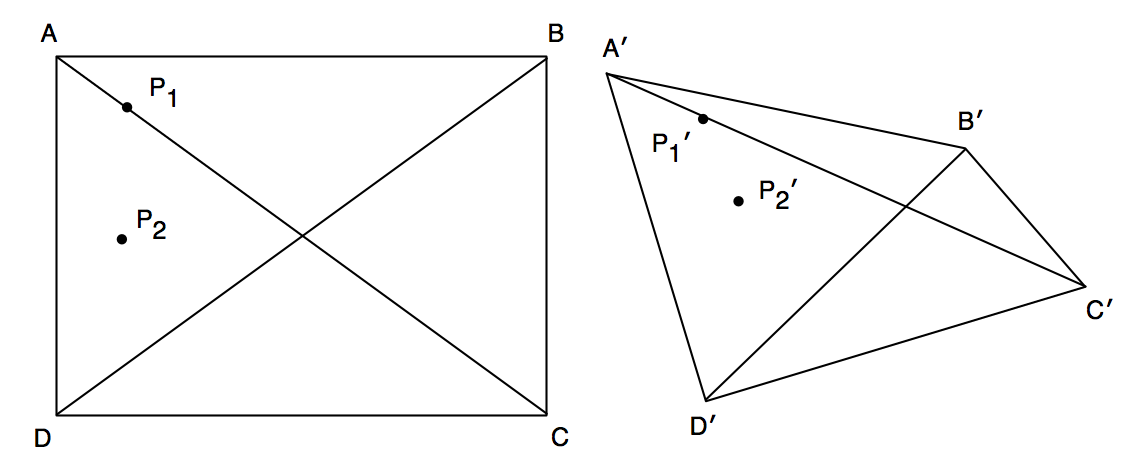
\includegraphics[width=0.65\textwidth]{images/arbiskew_graphic.png}
\caption{\emph{A visual representation of the result of the {\tt projective\_transform} module. Input is on the left, a possible output, for four coordinates $A\prime$, $B\prime$, $C\prime$, and $D\prime$ is on the right.}}
\end{figure}

Mathematically, the algorithm works as follows:
\begin{enumerate*}
\item Calculate the distance of line $\overline{A\prime D\prime}$ and assign it to $d_{ad}$.
\item Do the same for $\overline{B\prime C\prime}$ and assign it to $d_{bc}$.
\item Create two ``iterator points,'' point $I_A$ and $I_B$ initially located at $A\prime$ and $B\prime$.
\item Let $o_x = 0$ and $o_y = 0$
\item Calculate the distance between the iterator points, assign it to $d_i$.
\item Create a third iterator point, $I_C$ at the location $I_A$.
\item Assign the pixel value of $I_C$ to pixel $(o_x, o_y)$ in the original image.
\item Move $I_C$ along line $\overline{I_A I_B}$ by an amo
unt $= \frac{d_i}{width_{original}}$.
\item Increment $o_x$.
\item Repeat steps 7--9 until $I_C = I_B$.
\item Move $I_A$ along line $\overline{A\prime D\prime}$ by an amount $= \frac{d_{ad}}{height_{original}}$.
\item Move $I_B$ along line $\overline{B\prime C\prime}$ by an amount $= \frac{d_{bc}}{height_{original}}$.
\item Increment $o_y$.
\item Repeat steps 5--13 until $I_A = D\prime$ and $I_B = C\prime$.
\end{enumerate*}

The Verilog implementation of this module has two types of submodules. The algorithm requires no multiplications, but several divisions. To perform divisions, a divider module, named {\tt divider}, was used that implemented a simple restoring division algorithm. \cite{restoring}

The {\tt LPF} module, which sends pixel data to the {\tt projective\_transform} module, has a five clock cycle delay on transmitted pixels. Because of this, up to five pixels can arrive at {\tt projective\_transform} while it is unable to write to memory, even after {\tt pt} has told {\tt lpf} to stop sending new data. Because of this, it was necessary to create a buffer to hold pixel data until it was able to be written to {\tt memory\_interface}. The {\tt shift18} module accomplishes this by using 18 {\tt SRL16E} 16 bit shift register primitive elements to a create an 18 bit wide shift register. By setting the address of the multiplexer associated with each {\tt SRL16E} element, the length of the shift register can be expanded and contracted easily.

\begin{figure}[h!]
\centering
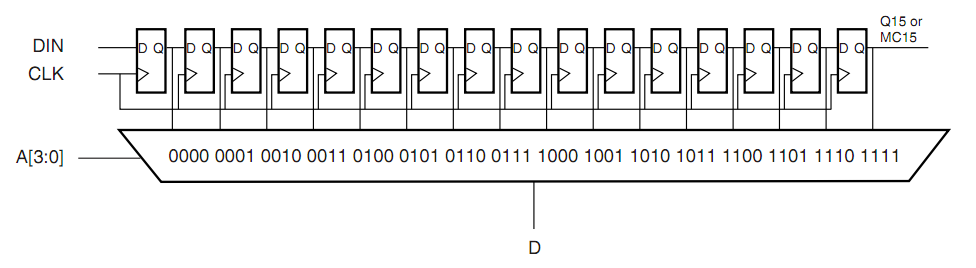
\includegraphics[width=\textwidth]{images/srl16.png}
\caption{\emph{The {\tt SRL16E} primitive shift register element. By setting {\tt A[3:0]}, the length of the buffer can be adjusted dynamically.}}
\end{figure}

\subsubsection{{\tt vga\_write} (Jos\'{e})}
% Jose
This module reads data from {\tt memory\_interface} and displays this data on the screen. Housed inside this module are (1) {\tt xvga}, which generates the VGA control signals necessary to display data on the screen, and (2) {\tt ycrcb2rgb\_lut}, which converts the fetched 18-bit YCrCb values to 24-bit RGB values suitable for display.

{\tt vga\_write} ``flags'' {\tt memory\_interface} and provides the interface the $(x,y)$ coordinates of the pixel to be displayed, which correspond to the hcount and vcount variables being output from the {\tt xvga} submodule. Because the {\tt xvga} module is clocked at 25MHz and {\tt memory\_interface} is clocked at 50MHz, care must be taken when requesting and reading pixels. Due to the implicit four-cycle delay of {\tt memory\_interface}, the outputs of {\tt xvga} must be delayed by two video clock cycles, so that the pixels that are output to the monitor correspond the control signals at the moment of ``flagging''. 

The fetched data consists of 36 bits, totalling two pixels. Every vclock cycle, the bits converted using {\tt ycrcb2rgb} are alternated between the higher-order 18 bits and the lower order 18 bits. The higher order 18 bits correspond to even pixels and the lower order 18 bits correspond to odd pixels. This set of control signals and pixel values is then pipelined, so that on the next rising edge these values are fed to the vga chip. The clock assigned to the vga chip (vga\_out\_clock) is an inverted copy of the onboard 25MHz clock, due to the high path propagation delay from the FPGA to the video DAC.

\paragraph{{\tt xvga}}
This submodule is an adapted version of the submodule used in the 6.111 Pong Lab. The adaptations include changing when the vsync, hsync, blank, and reset signals trigger based on the change of resolution from 1024x768 to 640x480. Operation involves a few basic steps\cite{xvga}: (1) Increment hcount by one every clock cycle, modulo 800. (2) Increment vcount by 1 when hcount has reached 799, modulo 524. (3) Pulse blank when either hcount $\geq 640$ or vcount $\geq 480$. (4) Pulse hsync when $656 \leq \text{hcount} \leq 752$. (5) Pulse vsync when $491 \leq \text{vcount} \leq 493$.

\paragraph{{\tt ycrcb2rgb\_lut}}
This submodule maps a YCrCb pixel to an RGB pixel. The mapping from YCrCb to RGB is summarized by the following set of equations\cite{ycrcb}:

\begin{align*}
R' & = 1.164(Y'-16) + 1.596(Cr-128) \\
G' & = 1.164(Y'-16) - 0.813(Cr-128) - 0.392(Cb-128) \\
B' & = 1.164(Y'-16) + 2.017(Cb-128)
\end{align*}

The luminance and chrominances have bitwidths of 8, 5, and 5, respectively. Initially, an approach with multipliers and adders was attempted. However, even with single and dual stage pipelining, we observed setup time violations due to the comparisons necessary to account for overflow and underflow caused by rounding error. As such, we opted to use look-up-tables to weigh Y, Cr, and Cb values and then to sum these weighted values to form the three different pixels. Because the contribution from luminance is identical for all colors, one lookup table with \( 2^8 \) entries was used for this factor. Lookup tables with \( 2^5 \) entries were used for the contributions from the chrominance values. Finally, adders were instantiated for adding all of these weighted factors. In the Appendix, you will find the code used to synthesize these LUTs, as well as the code for this module.

\section{Debugging and Testing}

Debugging and testing Verilog-defined hardware is complicated by extremely lengthy synthesis and implementation times. Because of this, we performed as much testing as possible in the ModelSim simulation environment. While ModelSim proved very fast and effective for ensuring that behavior logic was correct, it failed to help us determine the source of many physical timing bugs, such as setup and hold time violations on communications with the external ZBT memories.

\subsection{Testing {\tt projective\_transform}}

To test {\tt projective\_transform}, a test jig was developed that provided the module with a list of input pixels, of linearly increasing luminance. The test jig also took the output of {\tt projective\_transform}, and saved it into an external file, along with the x and y coordinates of each output pixel. A MATLAB script was then used to display the results of {\tt projective\_transform}, along with the original image. The result of this MATLAB script is shown below. In this way, the algorithm used by {\tt projective\_transform} to distort the image was known to be correct.

\begin{figure}[h!]
\centering

\includegraphics[width=0.4\textwidth]{images/original.png}
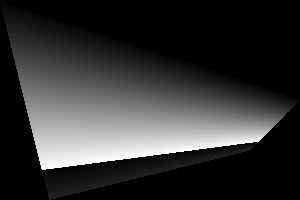
\includegraphics[width=0.4\textwidth]{images/output.png}
\caption{\emph{On the left, the sample input image used to test {\tt projective\_transform}. On the right, the output image from the testbench.}}
\end{figure}

 
\section{Conclusion}

\begin{thebibliography}{9}

\bibitem{restoring}
  Malek, Miroslaw.
  2002.
  \emph{Division algorithms.}
  Available: \\ \begin{url} http://devel-rok.informatik.hu-berlin.de/svn/TI2/2006/folien/pdf/eng\_ca12.pdf \end{url}

\bibitem{xvga}
  http://web.mit.edu/6.111/www/f2011/index.html [REFORMAT ME]

\bibitem{ycrcb}
  XAPP283: Color Space Converter (http://www-mtl.mit.edu/Courses/6.111/labkit/appnotes/xapp283.pdf) [REFORMAT ME]

\end{thebibliography}


\end{document}
